
\documentclass[times, 11pt,twocolumn]{article} 
\usepackage{latex8}
\usepackage{times}
\usepackage[ngerman]{babel}
\usepackage{todonotes}
\usepackage[utf8]{inputenc}
\usepackage{graphicx}
\usepackage[hyphens]{url}
\usepackage{mathtools}
\usepackage{amsmath}
\usepackage[font=small,labelfont=bf]{caption}

\pagestyle{empty}


\begin{document}

\title{Neuronale Netze in der Videoproduktion}

\author{Laura Anger\\
Technische Hochschule K\"oln \\ Institut f\"ur Medien- und Phototechnik \\  laura.anger@th-koeln.de \\
\and
Vera Brockmeyer\\
Technische Hochschule K\"oln \\ Institut f\"ur Medien- und Phototechnik \\ vera.brockmeyer@smail.th-koeln.de \\
}

\maketitle
\thispagestyle{empty}


\large{\textbf{Zusammenfassung}}\\ \small %\normalsize
\todo[inline, color=red]{Vera} 

\large{\textbf{Schl\"usselw\"orter}}\\ \small %\normalsize
 Faltungsnetze, Videoproduktion, Stilsynthese, Bewegtbildgenerierung, Deep Writing
 \todo[inline, color=red]{Vera} 


\Section{Einleitung} \label{sec:Einleitung}
\todo[inline, color=yellow]{Vera} 
Die Videoproduktion konnte sich im Zuge der Digitalisierung im letzten Jahrzehnt enorm qualitativ verbessern. Jeder der vier Produktionabschnitte (siehe Abbildung~\ref{fig:Videoproduktion}) konnte verbessert und nachhaltig erleichtert werden. In der Konzeptionsphase konnten die Arbeitsprozesse mit Hilfe des Internets erleichtert werden durch den beschleunigten weltweiten Austausch von Skripten oder den standort-unabhängigen Zugriff auf cloudbasierte Projektmanagement Systeme.

Während der Produktion des Videomaterials unterstützen moderne digitale Kamerasysteme den Kameramann indem sie den Weißabgleich und die Belichtung automatisch berechnen und einstellen. Selbst geringfügige unruhige Bewegungen werden mit Bildstabilisatoren direkt unterdrückt.  \textcolor{red}{Bin wohl echt n Phototechniker :-D Hast du evtl. n Tipp für z.b. vernetze Produktionssysteme}

Die darauffolgenden Arbeitsprozesse, wie das Schneiden und Editieren des Videomaterials währen der Postproduktionsphase, wurden in den letzten Jahren vereinfacht oder können teilweise durch zuverlässige Algorithmen automatisch durchgeführt werden. Mittlerweile können realistisch virtuelle Bildinhalte von \textit{Computer Generated Imaging} (CGI) Experten mit entsprechender Rechenkapazität in das gedrehte Videomaterial nahtlos rendert werden. Dies ermöglicht es Produktionen fast ausschließlich im Studio zu produzieren und sogar aufwendige Fantasywelten oder aufwendige Stunts mit geringeren Kosten umzusetzen.

Doch gerade qualitativ hochwertige Videoproduktionen erfordern immer noch einen sehr hohen Arbeitsaufwand mit einer große Anzahl an professionellen Mitarbeitern und kostenaufwändigen Materialien. Einen großen Anteil daran hat die Postproduktion in der jede Szene separat editiert und an das Gesamtbild angepasst werden muss. Dieses Gesamtbild muss vorab genau festgelegt werden, denn eine spätere Korrektur erfordert eine vollständige Wiederholung der meisten Arbeitsschritte. Aber auch die Generierung von Bildmaterialien für kurze Schnittszenen oder Webvideos ist sehr zeitaufwändig und kostenintensiv. Ein mehrköpfiges Team mit dem umfangreichen Equipment muss zum Drehort gebracht werden und unter Umständen auch untergebracht werden. Auch äußere Einflüsse, wie zum Beispiel das Wetter, können den Zeitplan verzögern und es entstehen zusätzliche Kosten. Für Studioaufnahmen muss in den meisten Fällen entsprechende Ressourcen angemietet oder auf Dauer gepflegt und in Stand gehalten werden.

In der Zukunft gilt es diesen Arbeits- und Kostenaufwand weiter zu reduzieren indem die einzelnen Arbeitsschritte automatisiert oder teil-automatisiert werden. Eine andere Vision ist es kurze Videoszenen für Webvideos oder Schnittszenen künstlich auf Basis von einzelnen Photographien am Computer zu erstellen. Dies erfordert Ansätze die komplexe Zusammenhänge und Erfahrungen wie das menschliche Gehirn vereinen können. Sie sollten im idealen Fall Kreativität umsetzen, Bewegungen und Abläufe voraussagen, bekannte Eigenschaften sinnvoll kombinieren oder erlernte Informationen übertragen und anwenden können. Diese Anforderungen können mit einer Form von künstlichen Intelligenz, den neuronalen Netzen (NN) (siehe Abschnitt~\ref{sec:Faltungsnetze}), erfolgreich erfüllt werden, die jenen des menschlichen Gehirn nachempfunden sind \cite{McCaigDG16}. In den letzten Jahren wurden NN stetig weiterentwickelt und es konnten vor allem im Bereich der Medienproduktion bahnbrechende Erfolge erzielt werden. Die vielversprechendsten Erfolge konnten mit einer besonderen Form der NN erzielt werden. Diese Faltungsnetze (CNN) (siehe Abschnitt~\ref{sec:Faltungsnetze}) ermöglichen orts- und skalierungs-unabhängige Operationen und somit ideal für mehrdimensionale digitale Signale.\\

Zu Beginn wurden CNN zur Objektklassifizierung eingesetzt um unter anderem automatisch Metadaten von Bild- oder Videodaten zu generieren und in Datenbanken oder Suchmaschinen einzupflegen. In den letzten Jahren wurden sie auch verstärkt für die Generierung oder Fortsetzung von bekannten Daten oder Signalen eingesetzt. Es konnten klassische Musikstücke sinnvoll beliebig verlängert werden~\cite{OordDZSVGKSK16} oder bewegte Sequenzen aus einzelnen Bildern generiert werden~\cite{Vondrick}. Auch in der Postproduktion konnten Bildern einer Stil aufgeprägt werden~\cite{DeepDream}. \\

In den folgenden Kapiteln wird in den Grundlagen (siehe Kapitel~\ref{sec:Grundlagen}) auf den allgemeine Ablauf in der Videoproduktion sowie detailliert die Funktionsweise der NN und CNN beschrieben. Im Anschluss werden in den folgenden Kapiteln verschiedene Entwicklungen von Videoproduktionsmittel vorgestellt, welche verschiedene Formen von NN und im besonderen von CNN nutzen. Drei Ansätze werden detailliert beschrieben und bewertet. Der erste Ansatz~\cite{Vondrick} beschreibt in Anschnitt~\ref{sec:Vondrick} die Generierung von eine bewegten Bildsequenz aus einem Einzelbild. Die anderen Ansätze~ \cite{DeepDream}~\cite{GatysEB15a} erläutert die Übertragung eines Bildstils auf eine andere Videosequenz.


\Section {Grundlagen} \label{sec:Grundlagen}
\todo[inline, color=yellow]{Laura} 
In Kapitel~\ref{sec:Videoproduktion} wird zunächst ein allgemeiner Überblick über die verschiedenen Arbeitsschritte einer Videoproduktion. Im drauf folgenden Kapitel werden die Grundlagen von NNs zusammengefasst. Um dann in Kapitel \ref{sec:Faltungsnetze} vertiefend auf Faltungsnetze einzugehen, deren Training in Kapitel~\ref{sec:Training} zusammengefasst wird. 
\SubSection{Videoproduktion} \label{sec:Videoproduktion}
\todo[inline, color=yellow]{Laura} 
Mit der Videoproduktion oder auch Filmproduktion wird die Herstellung sowohl von Kino- als auch von Werbe- und Fernsehfilmen zusammengefasst. In Abbildung~\ref{fig:Videoproduktion} ist ein Ablaufplan einer typischen Videoproduktion zu sehen. Da es alleine in Deutschland über 850 Produktionsformen gibt~\cite{formatt} (Stand 2014), kann der Ablaufplan nur einen sehr allgemeinen Überblick über die notwendigen Arbeitsschritte bieten. \\
Der erste Schritt, die Konzeption soll sowohl die Projektentwicklung, als auch die Vorproduktion zusammenfassen. Die sich anschließende Produktionsphase kann grob, wie im Schaubild zu sehen in Bild und Ton unterteilt werden, wobei diese beiden Bereiche nicht immer getrennt betrachtet werden sollten. Die Postproduktion besteht aus vielen verschiedenen Arbeitsschritten, deren Schwerpunkt auf dem Schnitt und der digitalen Bildnachbearbeitung liegt. Der Schritt der Distribution ist hier der Vollständigkeit halber erwähnt und beschreibt die Filmverwertung. \\

Der Aufbau der folgenden Ausführungen orientiert sich an Abbildung~\ref{fig:Videoproduktion} (vgl. Kapitel~\ref{sec:Konzeption},~\ref{sec:Produktion} und~\ref{sec:Postroduktion}).


\begin{figure}
	\flushleft
	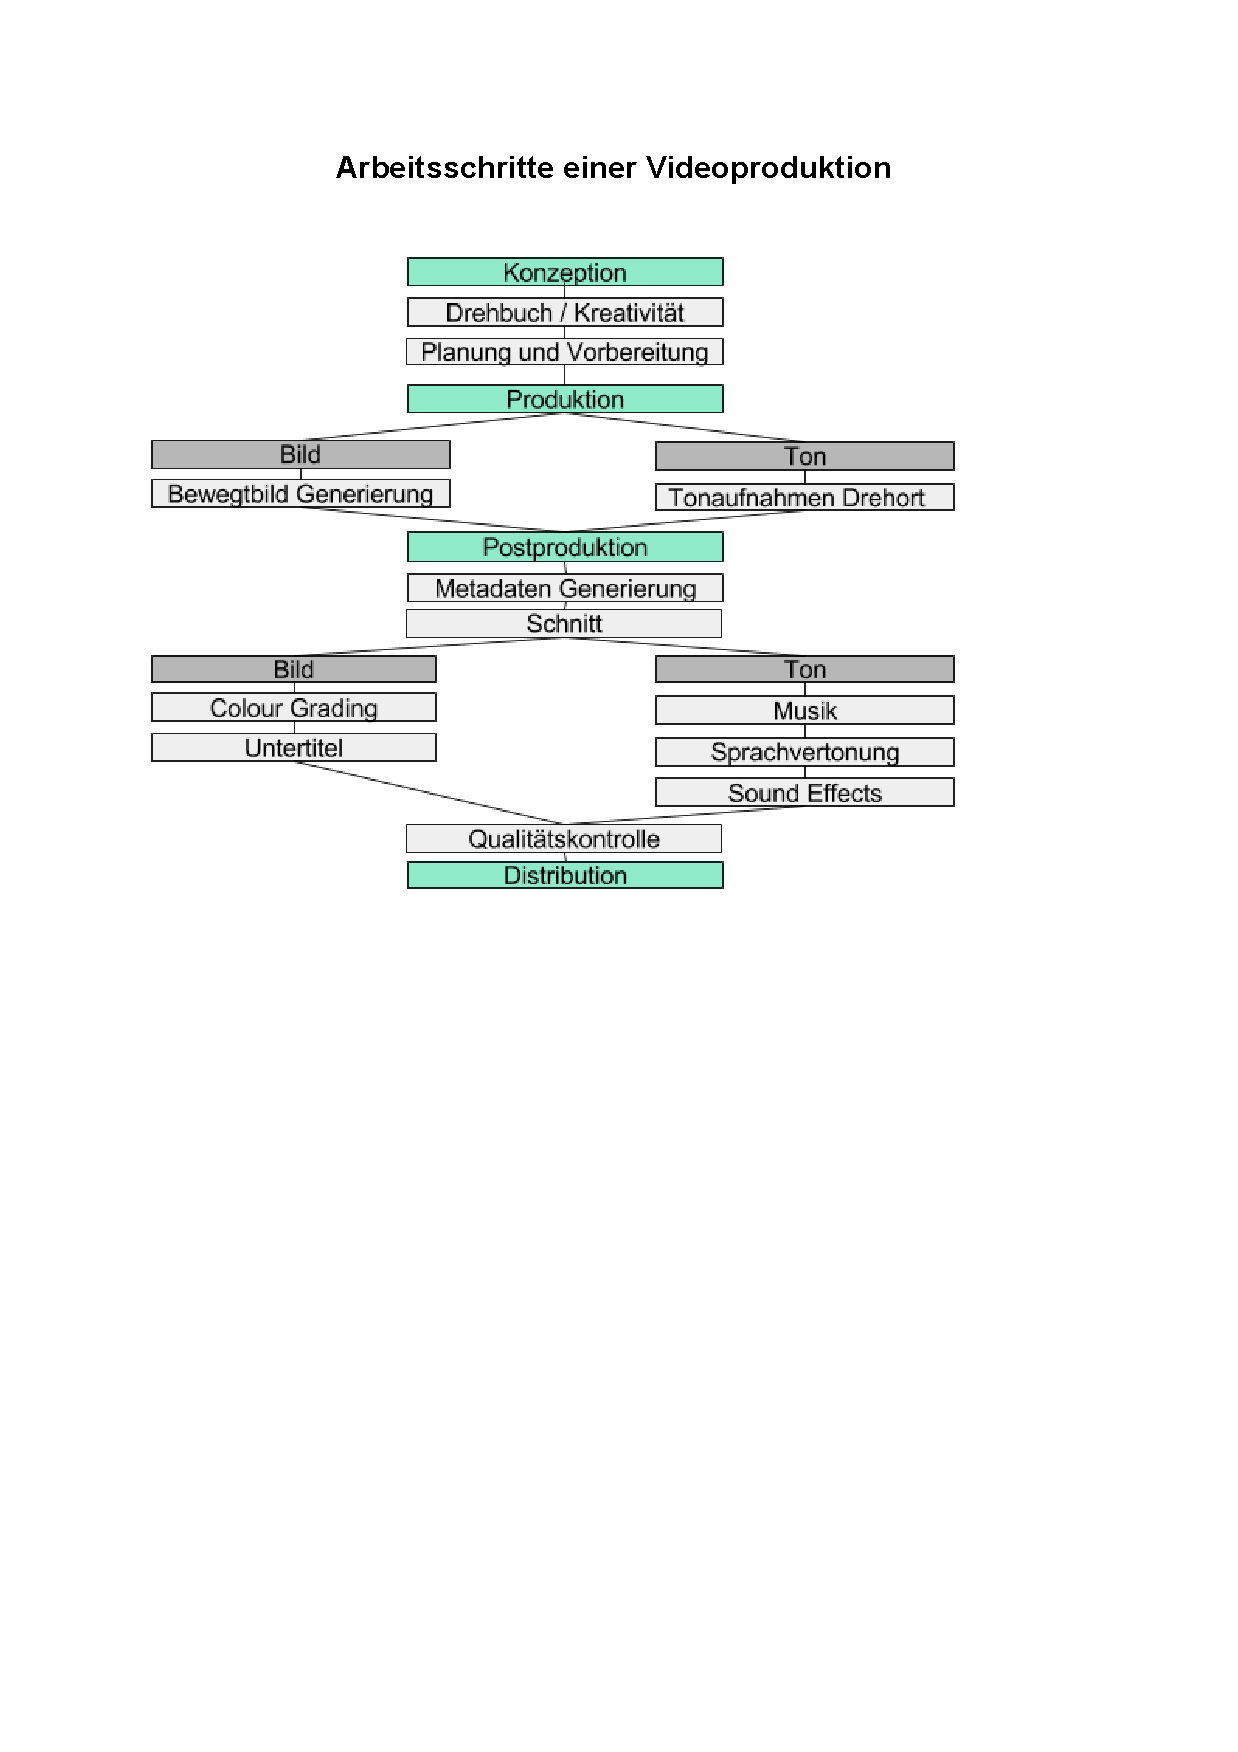
\includegraphics[width=\columnwidth, trim = 20mm 145mm 45mm 40mm, clip]{Bilder/ArbeitsschritteVideoproduktion.pdf}
	\caption{Grundlegende Arbeitsschritte einer Videoproduktion.}
	\label{fig:Videoproduktion}
\end{figure}
\SubSection{Neuronale Netze} \label{sec:NeuronaleNetze}
\todo[inline, color=yellow]{Laura} 

NNs finden unter anderem Anwendung bei der Steuerung von Robotern, Börsenkursanalysen, Medizin oder Fahrzeugsteuerung. In der Bildverarbeitung werden NNs vor allem zur Klassifizierung genutzt. \\
Sie sind vom menschlichen Gehirn inspiriert, welches laut \cite{NNHaykin} ein nicht-lineares, komplexes und hoch paralleles System zur Verarbeitung von Informationen darstellt. Ähnlich wie dieses bestehen künstliche NNs aus einer Menge an simulierten Neuronen, die untereinander verbunden sind und in Schichten organisiert sind. Es gibt verschiedene Arten der Vernetzung, die, wie in \cite{NNHaykin} und \cite{NNStanley} beschrieben, in rück- und vorwärts gekoppelte Modelle unterteilt werden können.\\

\begin{figure}
	\flushleft
	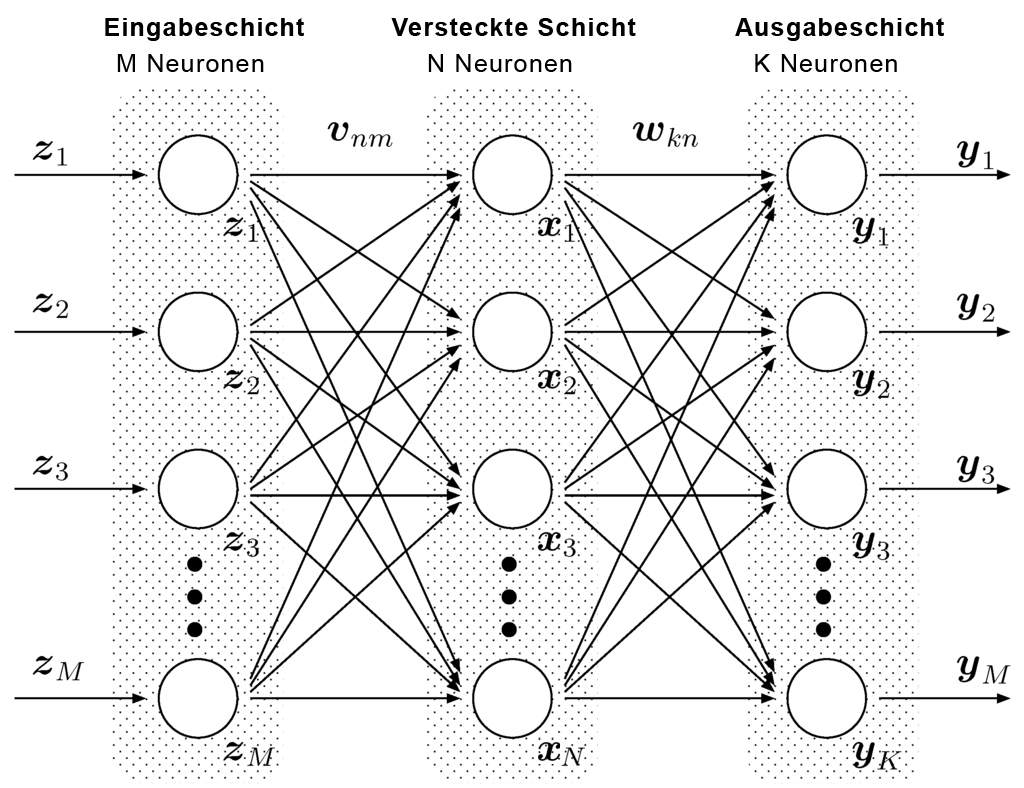
\includegraphics[width=\columnwidth]{Bilder/structure-mlp.jpg}
	\caption{Prinzipieller Aufbau MLP nach~\cite{MDPI}.}
	\label{fig:MLP}
\end{figure}

Am häufigsten kommen sogenannte \textit{Multilayer Perceptrons} (MLP)  \cite{NNBraun}\cite{NNNauck}\cite{NNStanley} zum Einsatz. Wie der Name vermuten lässt, werden hierbei die Neuronen in Schichten angeordnet. Ein solcher Aufbau ist beispielhaft in Abbildung~\ref{fig:MLP} zu sehen. Dieses MLP besteht aus eine Eingabe- und Ausgabeschicht mit $M$ bzw $K$ Neuronen und einer versteckten Schicht mit $N$ Neuronen. Es handelt sich um ein vorwärtsgekoppeltes Modell, bei welchem jedes Neuron einer Schicht mit jedem Neuron der darauffolgenden Schichte verbunden ist. Dies nennt man volle Verbindung. Die Eingangsschicht dient zum Verteilen der Eingangswerte $z_m$ mit $m=1,...,M$. Die Ausgabe eines jeden Neurons in der versteckten Schicht, dargestellt durch $x_n$, lässt sich durch Formel \ref{eq:AusgabeVerdeckteSchicht} berechnen. Hierbei steht $v_{nm}$ für die jeweilige Gewichtung der Verbindungen zwischen den Neuronen der Eingabe- und der versteckten Schicht und $f$ für die Aktivierungfunktion~\cite{NNStanley}\cite{NNHaykin} des jeweiligen Neurons. 

\footnotesize
\begin{equation} 
x_n = f~(\sum_{m=1}^M v_{nm}z_m)
	\label{eq:AusgabeVerdeckteSchicht}
\end{equation}
\small

Die Ausgangswerte $y_k$, mit $k=1,...,K$, lassen sich äquivalent unter Hereinnahme der Werte $x_n$ und der Gewichte $w_{kn}$, sowie einer Aktivierungsfunktion $g$ berechnen, und gelten als Vertrauenswerte. Sie müssen gemäß der Aufgabenstellung interpretiert werden. 


\SubSection{Faltungsnetze} \label{sec:Faltungsnetze}
\todo[inline, color=yellow]{Laura} 
Im Folgenden wird genauer auf Faltungsnetze eingegangen, da diese die Grundlage, für die meisten der in den folgenden Kapiteln vorgestellten Ansätze, bilden. Vereinfacht ausgedrückt besteht ein Faltungsnetz aus einer Vernetzung von Faltungsoperationen mit unterschiedliche Filtermasken. Faltungsnetze kommen, bedingt durch ihre Architektur, oft zum Einsatz, wenn große Datenmengen von einem NN verarbeitet werden sollen. Ein schematischer Aufbau ist in Abbildung~\ref{fig:CNN} zu sehen. 

\begin{figure}
	\flushleft
	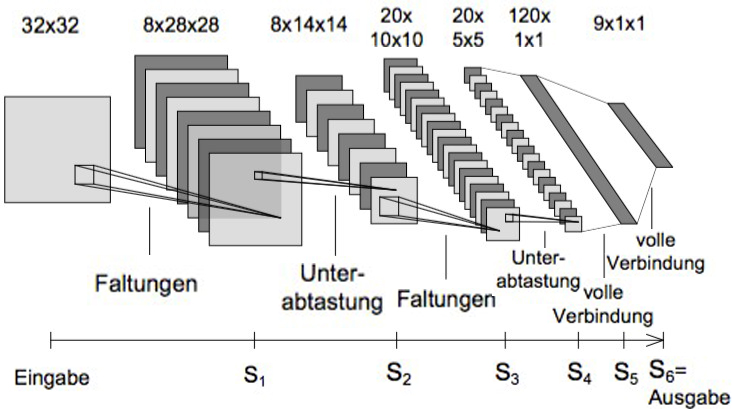
\includegraphics[width=\columnwidth]{Bilder/structure-cnn.jpg}
	\caption{Prinzipieller Aufbau Faltungsnetz nach~\cite{Osadchy}.}
	\label{fig:CNN}
\end{figure}

Jedes Pixel eines Feldes, das auf der Abbildung zu sehen ist, wird durch ein Neuron repräsentiert. Die Felder sind in Schichten organisiert. Die Eingangsschicht fungiert, vergleichbar wie bei den MLPs aus Kapitel~\ref{sec:NeuronaleNetze}, als Verteiler der Information an die Neuronen der nächsten Schicht $S_1$. Die Besonderheit eines Faltungsnetzes sind die sich abwechselnd durchgeführte Faltung und anschließende Unterabtastung. Zwischen den Schichten $S_4$ und $S_6$ ähnelt das Modell einem MLP, da die Neuronen schichtweise voll verbunden sind.\\

Im Allgemeinen wird für eine Faltung eine Filtermaske $h$, also eine endlicher zweidimensionaler Koeffizientensatz, wie in Formel~\ref{eq:Filtermaske} zu sehen, verwendet. Hierbei stehen $x$ und $y$ jeweils für die horizontale bzw. die senkrechte Bildkoordinate. Die Anzahl der Koeffizienten $a_{xy}$, wird in der Horizontalen mit $N_{hx}$ und im Vertikalen mit $N_{hy}$ bezeichnet. 

\footnotesize
\begin{equation} 
	h(x,y) = \left\lbrace
  \begin{array}{l@{}l}
   0~f\ddot{u}r~x<-\lfloor\frac{N_{hx}-1}{2}\rfloor~\vee~y<-\lfloor\frac{N_{hy}-1}{2}\rfloor\\
    0~f\ddot{u}r~x>\lfloor\frac{N_{hx}-1}{2}\rfloor~~~~\vee~y>\lfloor\frac{N_{hy}-1}{2}\rfloor \\
    a_{xy}
  \end{array}
  \right.	
	\label{eq:Filtermaske}
\end{equation}
\small  

Formel~\ref{eq:Faltung} beschreibt die Faltung eines Eingangssignals $s$ mit einer Filtermaske $h$, wobei I das Ausgangssignal in Abhängigkeit von $x$ und $y$ beschreibt.

\footnotesize
\begin{equation}
\begin{aligned}
I(x,y) = (s*h)(x,y) = \\
\sum_{m_x=-\infty}^\infty \sum_{m_y=-\infty}^\infty s(m_x,m_y) \cdot h(x-m_x,y-m_y) 
\end{aligned}
	\label{eq:Faltung}
\end{equation}
\small

Im Fall eines Faltungsnetzes wird die Faltung, die wie in Abbildung~\ref{fig:CNN} zu sehen, beispielsweise zwischen der Eingangsschicht und $S_1$ vollzogen wird, wird durch die Verbindung zwischen den Neuronen zweier Felder modelliert. Dabei entsprechen die Gewichte der Neuronen genau den Filterkoeffizienten $a_{xy}$. Für ein jedes Feld sind diese Koeffizienten konstant, was bedeutet, dass alle Neuronen eines Feldes mit nur einem Gewicht auskommen. Dieses Prinzip nennt man geteilte Gewichte. \\

Im Faltungsnetz wird nach jeder Faltung eine Unterabtastung durchgeführt um zu gewährleisten, dass die Dimension der Eingangsdaten schrittweise an die Dimension des Ausgangsvektors angepasst wird. Hierzu wird meist eine bilineare Unterabtastung um den Faktor 2 vorgenommen. Allgemeiner betrachtet werden $n$x$n$ Werte zu einem Wert zusammengefasst.\\

Wie zu Beginn des Kapitels erwähnt, haben Faltungsnetze gegenüber den MLPs den Vorteil, dass sie nahezu beliebig hochskaliert werden können und somit gut geeignet für große Datenmengen sind. Dies liegt vor allem daran, dass die Neuronen nur lokal verbunden sind und sich somit das Prinzip der geteilten Gewichte zu Nutze gemacht werden kann. Ein weiterer Vorteil von Faltungsnetzen, der vor allem in der Bildverarbeitung genutzt wird, ist das sie translationsinvariant sind.

\SubSection{Training Faltungsnetze} \label{sec:Training}
\todo[inline, color=yellow]{Laura} 
Meistens werden Faltungsnetze mittels der \textit{back-propagation} Methode trainiert. Bei dieser überwachten Lernmethode bedarf es einer großen Menge an vorher klassifizierten Eingabematerialien~\cite{5537907}. \\
In den Faltungsschichten kann der Fehler der vorangegangen Schicht nach Formel \ref{eq:Training} berechnet werden. Dabei steht $E$ für den Fehler in der jeweiligen Schicht $l$. Während $x^l$ für die Eingabe in die Schicht steht, bezeichnet $y^l$ die Ausgabe der entsprechenden Schicht. Die Größe der Eingabe wird der Einfachheit halber als quadratisch, also $mxm$-groß angenommen. Eine Gewichtung wird mit $w$ bezeichnet. für Um die Formel in der Realität anzuwenden, muss die linke und obere Grenze des Eingabeinhaltes, z.B. eines Bildes, mit Nullen ergänzt werden. Ansonsten wäre es nicht möglich den Fehler für Pixel zu berechnen, welche näher als $m$ an den entsprechenden Rändern liegen. 

\footnotesize
\begin{equation}
\begin{aligned}
\frac{\delta E}{\delta y_{ij}^{l-1}} = \sum_{a=0}^{m-1} \sum_{b=0}^{m-1} \frac{\delta E}{\delta x_{(i-a)(j-b)}^{l}} \frac{\delta x_{(i-a)(j-b)}^{l}}{\delta y_{ij}^{l-1}}  \\
= \sum \limits_{a=0}^{m-1} \sum \limits_{b=0}^{m-1} \frac{\delta E}{\delta x_{(i-a)(j-b)}^{l}} w_{ab}
\end{aligned}
	\label{eq:Training}
\end{equation}
\small

Die Schichten, in denen die Unterabtastung stattfindet, leisten kaum Beitrag zum eigentlichen Lernprozess des Faltungsnetzes. Hier wird das Problem allerdings reduziert, da $n$x$n$ Werte in einem einzigen resultieren. \\
Weil alle Gewichtungen mittels des \textit{back-propagation} Algorithmus während des Trainings angepasst werden, können Faltungsnetze laut LeCun als Erzeuger ihrer eigenen Merkmalextraktion gesehen werden \cite{LeCun:1998:CNI:303568.303704}.








\Section{Konzeption} \label{sec:Konzeption}
\todo[inline, color=yellow]{Vera} 
Vor der eigentlichen Produktion von Videomaterial muss das Projekt zunächst konzipiert und detailliert geplant werden. Dies bezieht sich vor allem auf die kreativen Prozesse des Drehbuchschreibens und die darauffolgende gesamte Projektplanung und -vorbereitung. Naturgemäß sind NN weniger sinnvoll für die Planung und das Management von Projekten. Doch in den letzten Jahren wurde damit begonnen mit Hilfe von NN kreative Prozesse umzusetzen und zu erforschen ob sie Kreativität entwickeln können. In diesem Sinne ist Kreativität auch mit sinnvollen und selbstständigem Denken sowie Entscheiden gleichzusetzen. Beides ist im Entstehungsprozess von Drehbüchern unumgänglich.

Es gibt bereits erste Versuche mit Hilfe von NN automatisch sinnvolle Texte und Dialoge zu erstellen, die auf bekannten Texten und Storylines basieren \cite{Thoma16}. Dieses Verfahren wird in der Literatur auch \textit{Deep Writing} genannt.Es können auch Romane, Dialoge oder Songtexte automatisch mit einem LSTM Recurrent NN erstellt werden~\cite{DrehbuchWrite}.

\SubSection{Aktueller Stand} \label{sec:SOTAVorverarbeitung}
\todo[inline, color=yellow]{Vera} 
Ein solches LSTM Recurrent NN wurde mit allen bekannten Episoden der Serie \textit{Silicon Valley} trainiert \cite{DrehbuchSV}. Nach dem erfolgreichen Training sind Wörter die häufig zusammenhängen in einem mathematischem Model gruppiert~\cite{DrehbuchWrite}. Zu Beginn des Schreibprozesses wird ein beliebiges Wort genutzt um den ersten Satz zu initialisieren. Das NN sucht im Anschluss das Wort, welches am häufigsten nach dem Startwort in den Trainingsdaten genannt wurde. Mit diesem Wortpaar wird nach dem selben Prinzip das dritte Wort des Textes ermittelt. Dieser Prozess wird solange wiederholt bis der generierte Text die gewünschte Länge erreicht hat.

Das Ergebnis sind Sätze, welche eine korrekte Grammatik aufweisen und häufig inhaltlich einen Sinn ergeben~\cite{DrehbuchSV}. Trotzdem ergeben die generierten Sätze beziehungsweise Dialoge sind nicht kohärent und folgen keiner ersichtlichen Storyline. \\

Der Film \textit{Sunspring}~\cite{DrehbuchMovie} wurde nach einem ähnlichen Prinzip erstellt und im Anschluss von einem professionellen Filmteam realisiert. Der größte Unterschied zu \cite{DrehbuchSV} ist, dass das NN nicht nur Wörter unterscheidet. Stattdessen wird zunächst alles in Buchstaben zerlegt und dann in neue Wörter und Sätze zusammengesetzt. Das verwendete NN nannte sich selber \textit{Benjamin} und wurde mit einer großen Anzahl an Drehbüchern von Science Fiction Filmen aus den 80er und 90er Jahren trainiert. 

Heraus kam ein Drehbuch, dass ähnlich wie \cite{DrehbuchSV} zwar grammatikalisch korrekte Sätze erschuf, die aber häufig inhaltlich keinen Sinn ergaben. Ein anderes Problem war der Umgang mit Namen, da diese sprachlich anders behandelt werden. Aus diesem Grund mussten alle Charaktere nur mit einzelnen Buchstaben benannt werden. Dies hatte zur Folge, dass das NN zwei Charaktere mit der selben Bezeichnung betitelt wurden und nachträglich umbenannt wurden.\\

Aus den mangelnden Zusammenhängen lässt sich ableiten, dass derzeit NN keine kreativen Prozesse simulieren können. Selbst mit einer sehr großen Anzahl von Trainingsdaten konnten keine kohärenten Dialoge generiert werden und keine konstante Storyline verfolgt werden. Weiterführend, sind die NN nicht in der Lage neue Charaktere oder Geschichten zu erfinden, sonder kombiniert lediglich bekannte wörtliche Zusammenhänge neu. Somit gibt es zur Zeit keinen brauchbaren Ansatz, welcher den Aufwand des Drehbuchschreibens minimieren könnte. 

\Section{Produktion} \label{sec:Produktion}
\todo[inline, color=red]{Laura} 
\textcolor{red}{muss angepasst werden} \\
In diesem Kapitel werden zunächst Ansätze vorgestellt, die auf Grundlage von NNs Arbeitsschritte bei der Produktion von Videos übernehmen bzw. vereinfachen könnten (vgl. Kapitel~\ref{sec:SOTAProduktion}). Dazu ist an zu merken, dass diese Ansätze meist in einem anderen Kontext entwickelt wurden und ggf. eine Anpassung an die Standards einer Produktion stattfinden müsste. \\

In Kapitel~\ref{sec:Vondrick} wird ein Ansatz zur automatisierten Generierung von Szenendynamiken in Hinsicht auf Funktionsweise und Arbeitserleichterung für die Videoproduktion analysiert. 


\SubSection{Aktueller Stand Musikgenerierung} \label{sec:SOTAProduktion}
\todo[inline, color=yellow]{Laura} 
Es gibt verschiedene Ansätze NNs zu nutzen, um Musik automatisiert generieren zu lassen. Im Folgenden werden drei Ansätze kurz vorgestellt, welche alle rückgekoppelte Neuronale Netze (RNN) benutzen. \\
An der \textit{University of Washington} ist im Rahmen einer Projektarbeit ein Musik Generator namens \textit{Algo Rythm} entstanden~\cite{Algorithm}. Für die Umsetzung habend die Studierenden um Timmerman RNNs geeignet trainiert. Der Quellcode kann auf Github \cite{AlgorithmGit} eingesehen werden.\\
Ein weiterer Ansatz, der in \cite{eck+lapalme:2008} beschrieben wird, arbeitet ebenfalls mit einem RNN, welches mit einem Autokorrelation-basierte Prädiktor kombiniert wird. Dabei soll die Struktur von Musikstücken erlernt werden, indem zunächst die folgende Note einer Tonreihenfolge vorausgesagt werden soll. \\
Der letzte Ansatz benutzt ebenfalls RNNs um auf Grundlage einer Notensequenz eine Musikstück zu komponieren \cite{browne2001system}. Dabei wird die Eingabesequenz zunächst interpretiert. Anschließend sorgen zwei RNN basierte Algorithmen für die Produktion von sowohl Rhythmus, als auch die Vorhersage der nächsten Note. \\

Alle drei Ansätze weisen hohes Potential auf, wenn es darum geht Musikstücke automatisiert zu generieren. Über das Genre des zugeführten Musikmaterials lässt sich die gewünschte Ausgabe begrenzt steuern. Es wäre durchaus vorstellbar, so Musik für eine Filmproduktion zu generieren.






\SubSection{Szenendynamik nach Vondrick et al.} \label{sec:Vondrick}
\todo[inline, color=red]{Laura} 
Mit dem Ansatz von Vondrick et al.~\cite{Vondrick} können aus Einzelbildern ganze Szenen Dynamiken erstellt werden, welche zum einen für die Klassifizierung und zum anderen für die Vorhersage von Bewegung genutzt werden kann. Das Resultat sind kleine Videos mit einer Auflösung von 65x64 Pixeln und 32 Einzelbildern. \\

Die Grundlage für dieses Verfahren bilden zwei Faltungsnetze, welche als Gegenspieler trainiert werden. \textit{Generative Adversarial Networks} (GAN) \cite{NIPS2014_5423} Dieses Konzept basiert auf einem Generator und Diskriminator und w
gegeneinander Trainieren siehe Formel (1)

unsupervised learning. 
Trainiert nach Kategorien



\begin{figure}
	\flushleft
	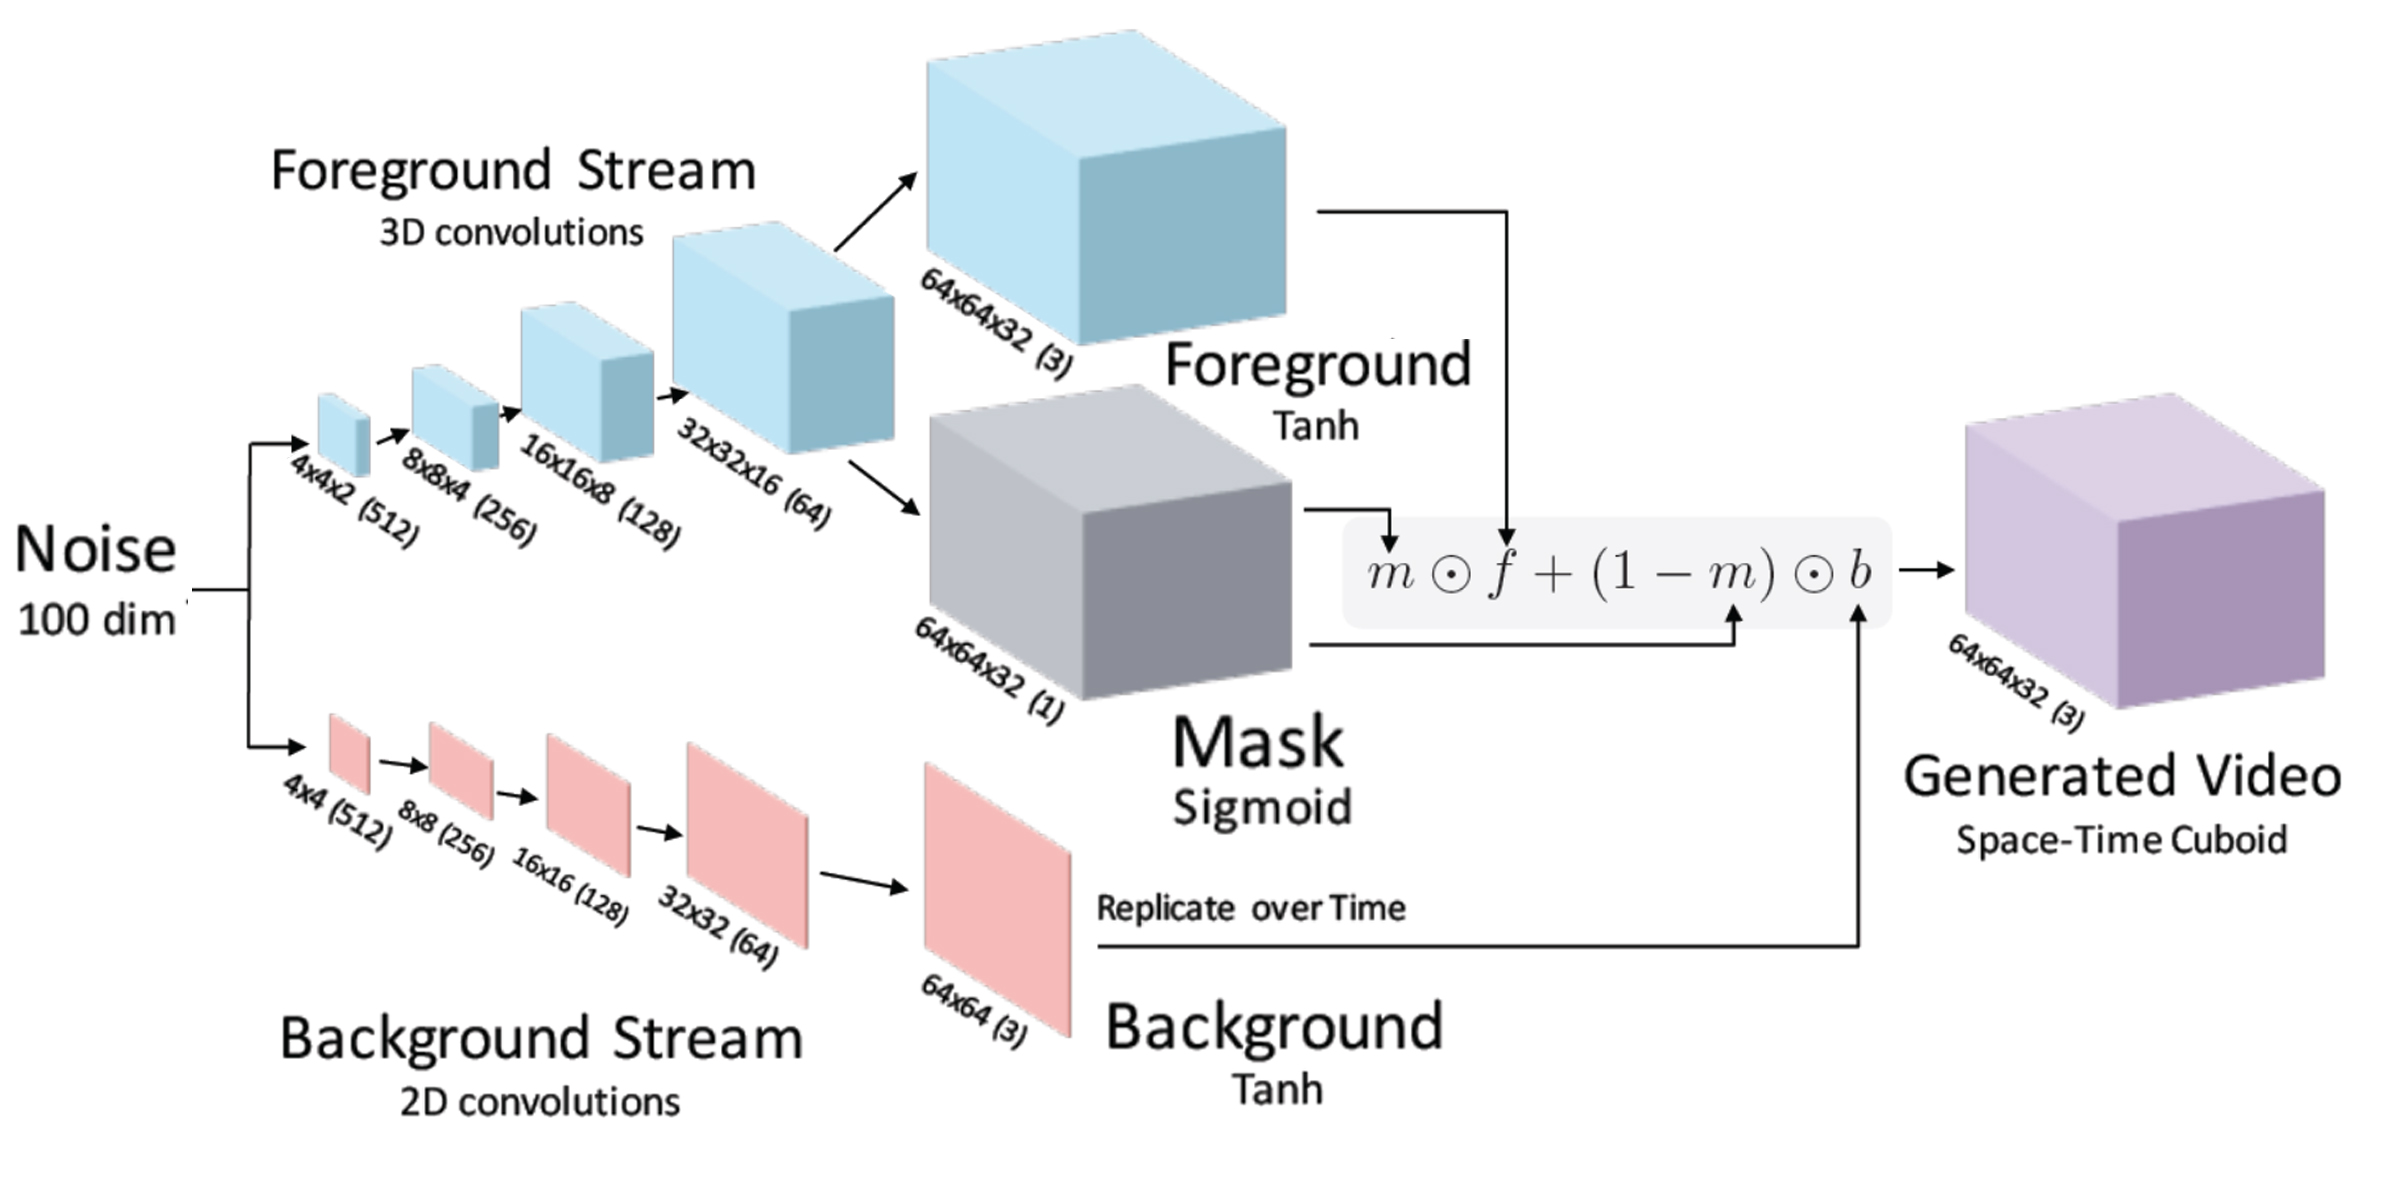
\includegraphics[width=\columnwidth]{Bilder/generator2.jpg}
	\caption{Aufbau Generator nach~\cite{Vondrick}.}
	\label{fig:generator}
\end{figure}


\begin{figure}
	\flushleft
	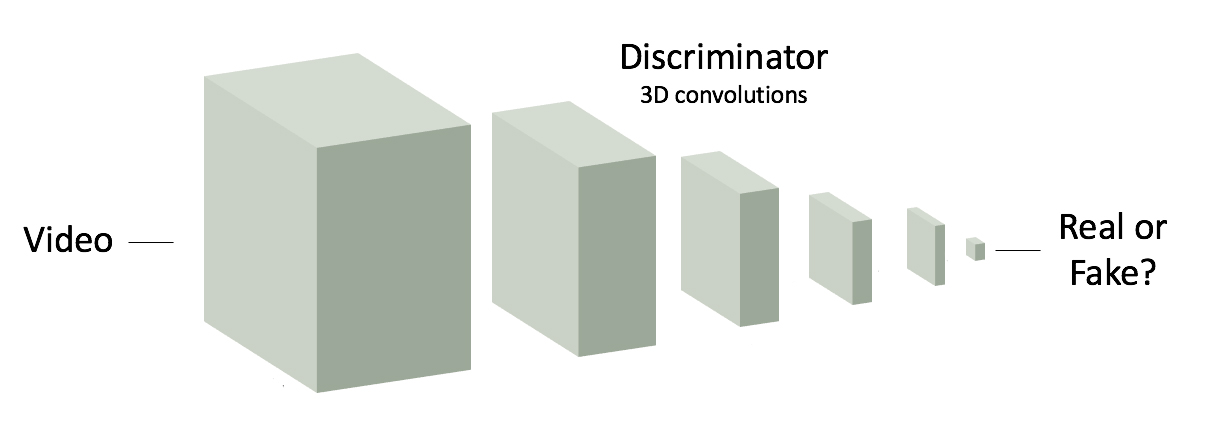
\includegraphics[width=\columnwidth]{Bilder/discriminator.jpg}
	\caption{Aufbau Diskriminator nach~\cite{Vondrick}.}
	\label{fig:discriminator}
\end{figure}

\begin{figure}
	\flushleft
	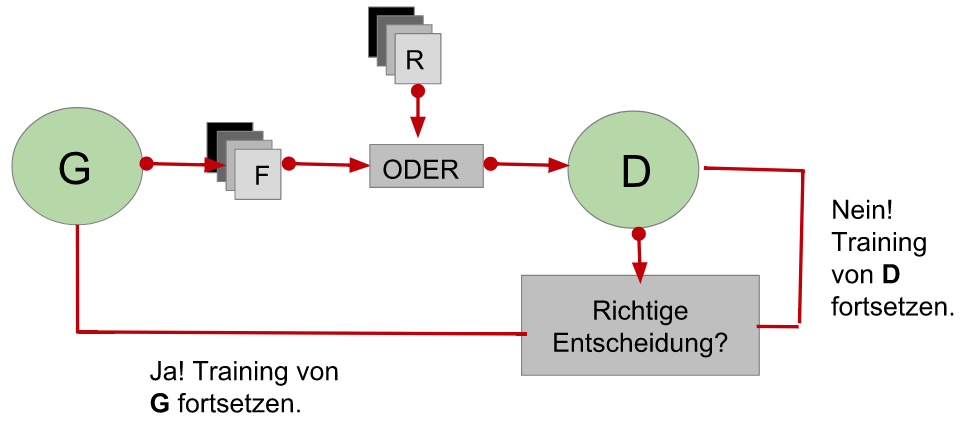
\includegraphics[width=\columnwidth]{Bilder/disAndGen.jpg}
	\caption{Zusammenspiel Diskriminator und Generator.}
	\label{fig:disAndGen}
\end{figure}




\SubSection{Bewertung des Ansatzes von Vondrick} \label{sec:VondrickConclusion}
\todo[inline, color=red]{Laura} 

Vorteile Verfahren:
- automatisierte Vorverarbeitung des Lernmaterials möglich
- Vorverarbeitung muss nur einmal gemacht werden
- Trainingsmaterial für G kann auch für D genutzt werden
- Bewegungen werden nach Kategorien gelernt

Vorteile in Bezug auf Videoproduktion:
- Verständnis der Szenen Dynamik wird wichtiger
- planen höhere Auflösung
- Denkbar für Realisierung von bspw. GIFs
- Simulationen oder Vorhersagen 

Nachteile:
- bedarf viel Trainingsmaterial
- Kategorien ohne Vernunft ausgewählt
- Realismusgrad nicht ausreichend
- Es gibt noch keine höhere Auflösung




\Section{Postproduktion} \label{sec:Postroduktion}
\todo[inline, color=yellow]{Vera} 

In diesem Kapitel wird die Verwendung von NN in der Videopostproduktion beschrieben. Gerade in diesem Produktionsabschnitt finden NN eine breites Anwendungsfeld, da gerade die CNN im Bereich der Bildverarbeitung in den letzten Jahre sehr erfolgreich eingesetzt werden konnten. Vor allem für die Bildklassifikation und Stilsynthese erweisen sich CNN als äußerst sinnvoll. Stilsynthese-Verfahren extrahieren idealerweise einen Bildstil und übertragen ihn sinngemäß auf ein weiteres unabhängiges Bild ohne den Bildinhalt zu modifizieren. Weiterführend stellte sich  heraus, dass CNN auch für \textit{Text-to-Speech} Verfahren erfolgreich eingesetzt werden können.\\

Im nächsten Abschnitt werden zunächst die interessantesten auf NN-basierenden Bildverabeitungs- und Text-to-Speech Ansätze in der Postproduktion vorgestellt und bewertet. Auf zwei Verfahren zur Stilsynthese wird in den darauffolgenden Anschnitten näher eingegangen inklusive einer ausführliche Analyse über die Verwendung der Verfahren in der professionellen Videoproduktion. Der zweite Ansatz ist eine Weiterentwicklung des ersten und somit bauen die Algorithmen aufeinander auf. Zuletzt wird ein Ausblick auf Einsatzmöglichkeiten gegeben.
.
\SubSection{Aktueller Stand} \label{sec:SOTAPostproduktion}
\todo[inline, color=yellow]{Vera} 
Für einige Produktionen, wie Dokumentationen oder Nachrichtensendungen, ist erforderlich sogenannte \textit{Voice-Over} auf das Videomaterial zu legen. Diese müssen vorab in einem Tonstudio mit einem Sprecher produziert werden. Dies kann zukünftig durch \textit{Text-to-Speech}- Verfahren ersetzt werden. Ein vielsagender Ansatz ist \textit{WaveNet}, welches im Gegensatz zu den meisten anderen Ansätzen auf einem CNN basiert~\cite{OordDZSVGKSK16}. Dieses CNN ist wie ein pixelbasiertes CNN aufgebaut. In das Netz werden textbasierte Eingangsdaten gegeben, welche vom CNN in Audiodaten gewandelt werden. Diese Audiodaten klingen mit Vergleich mit anderen bekannten Verfahren nahezu fehlerfrei und natürlich. Die generierten Audiodaten werden fast als menschliche Stimme wahrgenommen. Doch verfahrensbezogen können nur Stimmen imitiert werden von denen vorab Stimmproben in das NN geben wurden.\\
Das \textit{Deep Voice} Verfahren~\cite{DeepVoice} baut auf dem \textit{WaveNet} Prinzip auf und entwickelt es weiter. Während \textit{WaveNet} mehrere Minuten Rechenzeit benötigt um eine Sekunde an Audiodaten zu generieren, ist \textit{Deep Voice} Realtime-fähig. Ein weiterer Vorteil ist, dass \textit{Deep Voice} ein eigenständiges System ist, welches es für die Nutzung in der Videoproduktion interessanter macht. Einen Vergleich bezüglich der Klangqualitätsunterschiede zwischen den beiden Verfahren gibt es leider nicht.
\\

Nachdem alle notwendigen Daten produziert wurden ist es der erste Schritt die Daten zu sichten, kennzeichnen und in entsprechende Mediendatenbanken für die weitere Produktion einzupflegen. Alle drei Schritte können mit Hilfe von NN erheblich automatisiert werden. Vorallem in der Objekterkennung und -klassifikation konnten mit CNN in den letzten Jahren eine sehr geringe Fehlerquote und hohe Robustheit erreicht werden. Aus diesem Grund werden sie flächendeckend in der Praxis verwendet. Eine bekannte Bibliothek ist \textit{Clarifai}~\cite{MITReview}, welche konfigurierte CNN anbietet um optimierte Bild- oder Videodatenbanken anzulegen und zu verwalten.  Weitere aktuelle Veröffentlichungen~\cite{Ng_VideoLabelling}\cite{Ye:VideoLabelling}\cite{KangEABZ17} konzentrieren sich auf die Verbesserung der Leistungsfähig um auch große Videodaten robust verarbeiten zu können. Dies ist für die große Menge an Videodaten einer Filmproduktion unbedingt notwendig. Zum jetzigen Zeitpunkt erfordert die Erkennung dieser Mengen noch sehr große Rechenkapazität und ist somit entsprechen kostenintensiv während sie dennoch Personalaufwand einspart. \\

Neben der verbreiteten Klassifikation können CNN auch Bilddaten generieren oder synthetisieren. Zwei vielversprechende Ansätze sind das Deep Dream~\cite{DeepDream} und das Deep Style Verfahren~\cite{GatysEB15a}. Ein großer Vorteil beider CNN-basierten Verfahren gegenüber den bekannten Synthese-Verfahren ist dass sie die gesamte Semantik eines Bildes vom Inhalt eindeutig zu trennen und mit einem unabhängigem Bild verschmelzen können. Bildlich gesprochen bedeutet dies, dass die  Verfahren den gesamten Stil eines Gemäldes mit der Farbwelt, dem Pinselstrich und dem Grad der Abstraktheit erfassen und übertragen können während die bekannten Verfahren nur einzelne Ausschnitte der Gemäldemerkmale erkennen. Hierfür ist es notwendig die höherwertigen Texturmerkmale des stilgebenden Bildes zu extrahieren und ein Zielbild so zu transformieren, dass es der extrahierten Semantik gleicht ohne dessen Bildinhalt zu verändern~\cite{McCaigDG16}. Dabei wird strikt zwischen den stilgebenden und inhaltsbezogenen Merkmalen unterschieden um eine Modifikation des Inhalts verhindern.

\SubSection{Faltungsnetze zur Stilsynthese}\label{sec:Stilsynthese}
\todo[inline, color=yellow]{Vera} 
Um die folgenden Algorithmen in Abschnitt~\ref{sec:DeepDream} und \ref{sec:DeepStyle} besser verstehen zu können muss zunächst näher auf die Prozesse innerhalb eines CNN eingegangen werden. In Abbildung~\ref{fig:CNN} wird deutlich, dass mit jeder weiteren Schicht das Bild stärker unterabgetastet wird und die Größe der Merkmalsvektoren stetig steigt. Mit jeder weiteren Schicht wird ein größer Ausschnitt des Bildes erfasst und dessen Merkmale extrahiert. Die Merkmalsvektoren werden größer, da ein größerer Bereich mehr Merkmale enthält und diese folglich immer komplexer werden. \\
Im oberen Bereich der Abbildung~\ref{fig:StyleRepresenation} wird veranschaulicht, dass mit steigender Schichtanzahl die stilgebenden Merkmale immer höherwertig werden und sich der Semantik des Stilbildes annähern. Während in der ersten Schicht die Stilmerkmale sehr klein sind und nicht der Bildsemantik ähneln, können in den höherwertigen Schichten Stilelemente aus dem gesamten Bild gefunden werden, wie zum Beispiel die gelben Kreise und die Strudel im Himmel. Im untereren Abbildungsbereich sind die inhaltsbezogenen Merkmale dargestellt. Hier ist die Unterabtastung klar zu erkennen und mit jeder Schicht wird die Darstellung der Merkmalsvektoren immer gröber. Trotzdem bleibt es stets erkennbar welches Gebäude abgebildet wird. Die Inhaltsinformationen bleiben demzufolge erhalten.\\

Gleichzeitig veranschaulicht die Abbildung~\ref{fig:StyleRepresenation}, dass die Inhalte der verborgenen Schichten eines trainierten CNN visualisiert werden können. Um dieses Wissen zu erlangen, wurden der übliche Prozess zur Objekterkennung invertiert. Das trainierte CNN wurde mit einem Eingangsbild initialisiert, welches ausschließlich zufälliges Rauschen enthält. Dieses Eingangsbild solange durch das CNN iteriert bis das gewünschte Objekt klassifiziert werden konnte. In diesem Bild konnten teilweise eindeutige Merkmale dieses Zielobjektes ausgemacht werden. An dieser Stelle sei hinzugefügt, dass das CNN ein Objekt nicht immer präzise bestimmen kann, da die Klassifikation stark von den Trainingsdaten abhängt. Zum Beispiel bei der Bestimmung von Hanteln kann es dazu kommen, dass auch Arme zum Merkmalsvektor hinzugefügt werden, da diese überdurchschnittlich häufig auf den Trainingsdaten mit den Hanteln zu sehen waren. Trotzdem führt dieser invertierte Prozess zu der Erkenntnis, dass CNN auch für die Generierung von Bilddaten genutzt werden und nicht ausschließlich für die Klassifizierung \cite{DeepDream}.\\
Ein anderer Ansatz lässt das CNN selbst entscheiden, welche Merkmale verstärkt werden. Das beliebige Eingangsbild wird durch das CNN propagiert und die Merkmalsvektoren der einzelnen Schichten untersucht. In den niedrigeren Schichten können nur primitive Texturmerkmale ausgemacht werden, wie Linien oder Rechtecke, während der Bildinhalt unverändert bleibt. Mit steigender Schichtanzahl werden die verstärkten Muster immer komplexer und der Bildinhalt wird teilweise modifiziert. So wird deutlich, dass CNN in den höheren Schichten die benötigten Informationen der Semantik enthalten und diese eindeutig vom Bildinhalt separiert werden können.\\
\begin{figure}
	\flushleft
	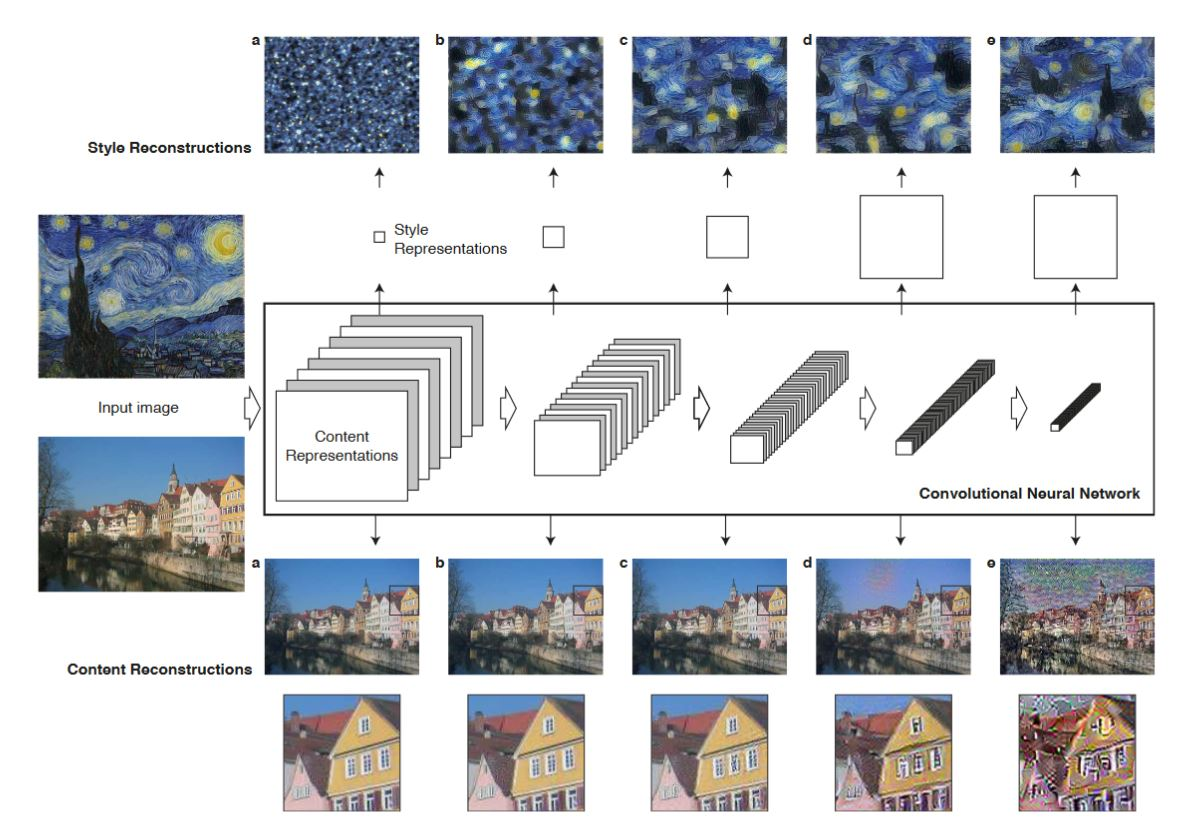
\includegraphics[width=\columnwidth]{Bilder/StyleRepesentation.JPG}
	\caption{Merkmalsextrahierung in einem Faltungsnetz\cite{GatysEB15a}.}
	\label{fig:StyleRepresenation}
\end{figure}

\SubSection{Deep Dream} \label{sec:DeepDream}
\todo[inline, color=red]{Vera} 
Der folgende Abschnitt stellt das Stilsynthese-Verfahren \textit{Deep Dream} \cite{DeepDream} vor, welches ein Nebenprodukt des Versuches den Inhalt eines CNN zu visualisieren ist. \textit{Deep Dream} basiert auf einem \textit{GoogLeNet} CNN mit 22 Schichten und fünf Unterabtastungsschichten~\cite{Szegedy_2015_CVPR}. Die Schichten haben eine besondere Architektur, welche \textit{Inception Layer} genannt wird. Mit Hilfe dieser Architektur können auch effizient große Merkmalsvektoren verarbeitet werden. Dieses \textit{GoogLeNet} wird im ersten Schritt mit dem \textit{\textit{ImageNet}} Trainingsdatenset trainiert.\\
An dieser Stelle sei zum besseren Verständnis hinzugefügt, dass ein wichtiger Unterschied zu den bereits bekannten Faltungsnetzmodellen aus Abschnitt~\ref{sec:Faltungsnetze} besteht. Die Schichten zur eigentlichen Klassifizierung sind für die Stilsynthese nicht relevant sind. Interessant sind die Faltungsschichten, welche die benötigten Merkmalsvektoren extrahierten und speichern.\\
Zunächst wird das stilgebende Bild, im folgenden Style Source (SS) genannt, bis zu einer beliebigen Schicht vorwärtspropagiert und der entsprechende Merkmalsvektor als $\vec{f_{GS}}$ gespeichert. Dieser enthält die Merkmale der gewünschten Semantik und steuert die Transformation in Richtung des gewünschten Stils. Würde $\vec{f_{GS}}$ entfallen nähert das CNN die Transformation an die Trainingsdaten an.  Bezogen auf Abschnitt\ref{sec:Stilsynthese} empfiehlt es sich höherwertige Schichten zu wählen um eine zufriedenstellendes Synthese zu generieren.\\
\begin{figure}
	\flushleft
	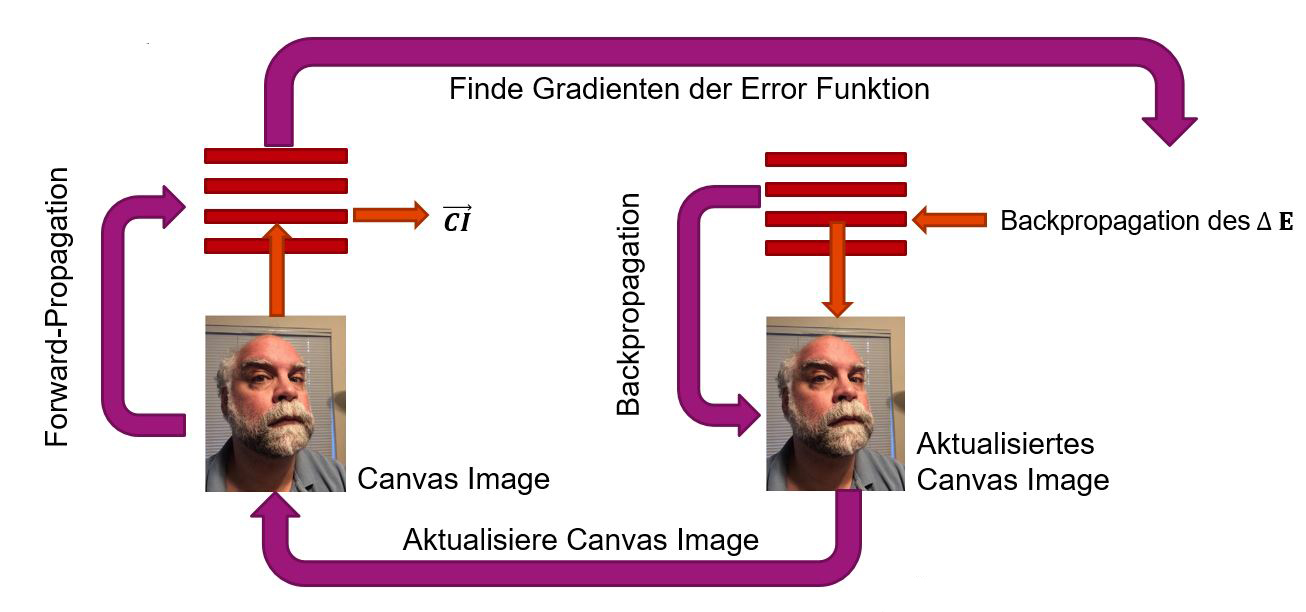
\includegraphics[width=\columnwidth]{Bilder/DeepDream.jpg}
	\caption{Ablaufdiagramm des Deep Dream Verfahrens.}
	\label{fig:DeepDream}
\end{figure}
Den weiteren Transformationsprozesses stellt Abbildung~\ref{fig:DeepDream} schematisch dar. Das Zielbild, im folgenden Canvas Image (CI) genannt, wird iterativ transformiert. Zu Beginn einer Iteration wird es bis zur selben Schicht wie $\vec{f_{CS}}$ vorwärtspropagiert und als $\vec{f_{CS}}$ gespeichert. Im Anschluss wird der Gradient der Fehlerfunktion $\Delta E(x,y)$ aus Gleichung~\ref{eq:DeepDreamError} berechnet. Diese ist als das Skalarprodukt aus $\vec{f_{CS}}$ und $\vec{f_{CS}}$ definiert, welches maximal ist, wenn beide Vektoren in die selbe Richtung zeigen.
\footnotesize
\begin{equation}
E(x,y)= \vec{f_{GS}}* \vec{f_{CS}}
\label{eq:DeepDreamError}
\end{equation}
\small
Der resultierende  $\Delta E(x,y)$ wird zurückpropagiert und die Gewichtungen innerhalb des Netzes in Richtung des SS korrigiert. Das daraus entstehende Bild wird als neues CI aktualisiert und für die nächste Iteration verwendet.
Dieser Ablauf wird solange wiederholt bis sich $\vec{f_{CS}}$  möglichst dem Ausgangsbild $\vec{f_{GS}}$ angenähert hat und der Fehler minimal ist. In diesem Fall ist $E(x,y)$ maximal und der gesamte Prozess wird als Maximierung von Gleichung~\ref{eq:DeepDreamError} interpretiert.\\

\begin{figure}
	\flushleft
	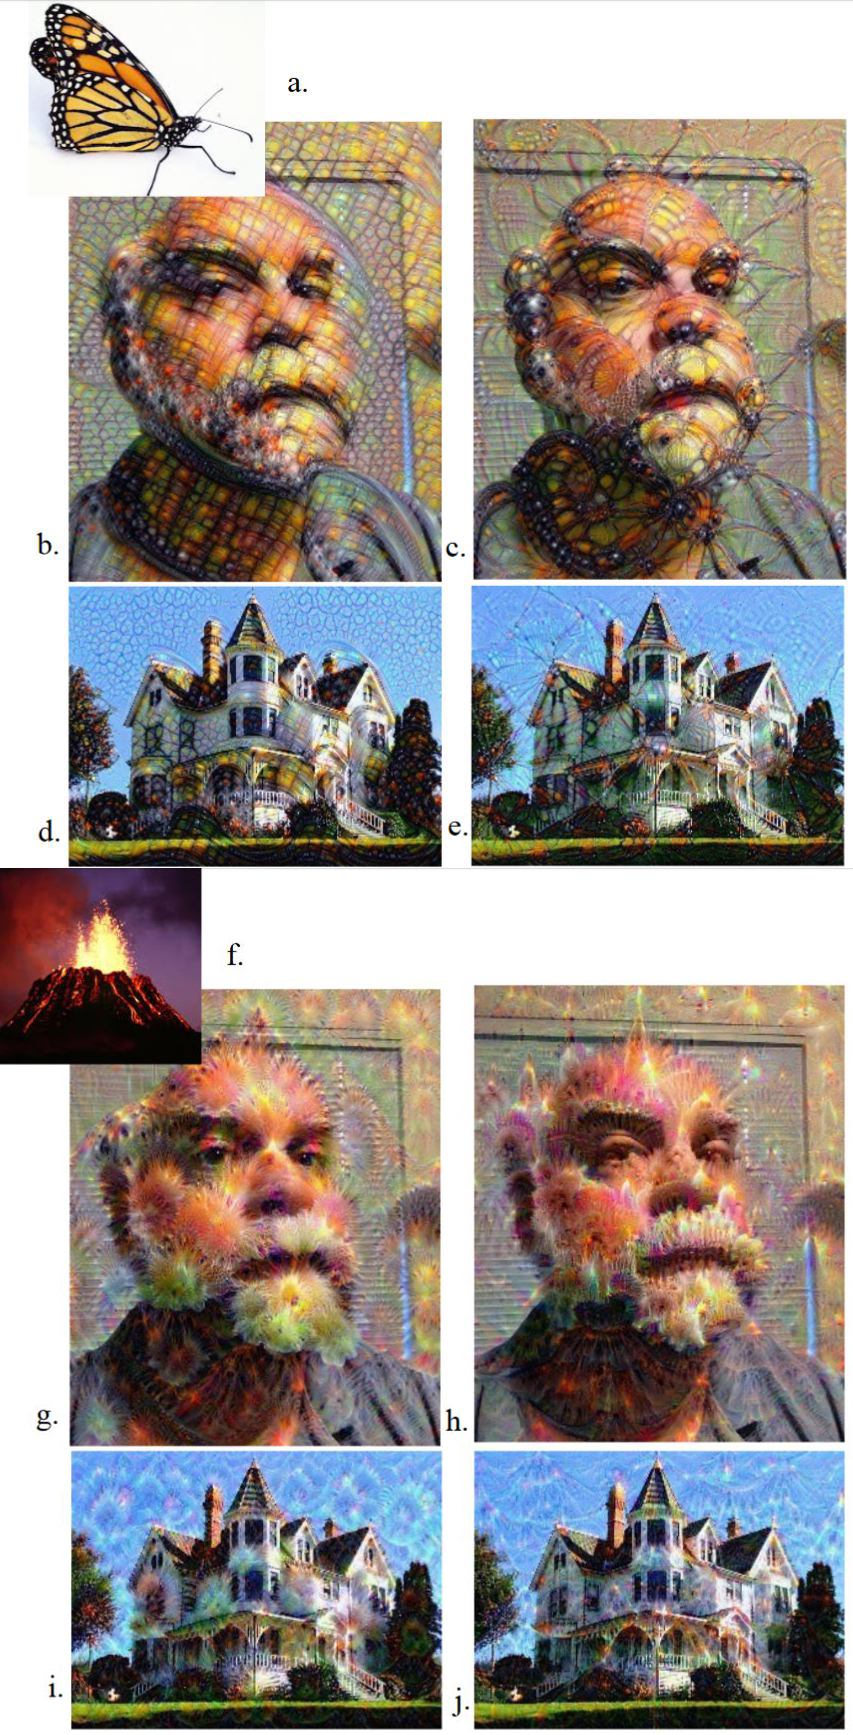
\includegraphics[width=\columnwidth]{Bilder/DeepDreamResults.JPG}
	\caption{Resultate des Deep Dream Verfahrens~\cite{McCaigDG16}.}
	\label{fig:DeepDreamResults}
\end{figure}

Einige Ergebnisse des \textit{Deep Dream} Verfahrens sind in Abbildung~\ref{fig:DeepDreamResults} dargestellt. Die kleinen Bilder in der oberen Ecke sind die verwendeten SS. Auf der linken Seite sind jeweils die Ergebnisse mit einer niedrigen Schicht und rechts solche einer höheren Schicht dargestellt. Auf den ersten Blick fällt direkt auf das die linken Bilder stärker die kleinen Merkmales übernommen haben während rechts eindeutig größere Texturen übernommen wurde, wie zum Beispiel die Form des Schmetterlings oder Vulkans am Hals. Gleichzeitig fällt rechts auf, dass markante Bildpunkte, wie die Augen oder die Nase, stark modifiziert wurden und teilweise sogar deren Form verändert wurde. Somit können teilweise Inhalte des ursprünglichen Bildes verloren gehen. Die Nase wurde in c einer Hundeschnauze angenähert, da die Trainingsdaten von \textit{ImageNet} einen Überschuss an Hundemotiven enthält. Besonders deutlich wird dies, wenn dein SS verwendet wird\cite{McCaigDG16}. Andere Ergebnisse zeigten auch deutlich, dass durchaus auch die Merkmale der Trainingsdaten gegenüber denen des SS überwiegen können.
\\
Es ist demzufolge für den Nutzer nicht möglich die Endergebnisse zu kontrollieren oder in den Prozess einzugreifen. Die einzige Möglichkeit der Kontrolle bietet die Wahl des SS und der Trainingsdaten, welche einen nicht vorhersehbaren Einfluss auf das Endergebnis haben. Daher kann von keiner strikten Trennung von Semantik und Inhalt ausgegangen werden. \\
Weiter kann nicht gewährleistet werden die Ergebnisse zu reproduzieren und ähnliche Bilder auf kohärente  Weise zu transformierten, da die Gewichte des CNN stetig während einer Iteration modifiziert werden. Diese Reproduzierbarkeit und Kohärenz ist ein wichtiges Kriterium für die Videoproduktion, da eine Sequenz von ähnlichen Bilder entsprechen gleichförmig transformiert werden muss. Aus diesem Grund ist dieses Verfahren mehr als neue Kunstform und interessante Spielwiese um die Funktionalität von CNN besser zu verstehen. Für die Videoproduktion ist sie gänzlich ungeeignet.



\SubSection{Deep Style}\label{sec:DeepStyle}
\begin{figure}
	\flushleft
	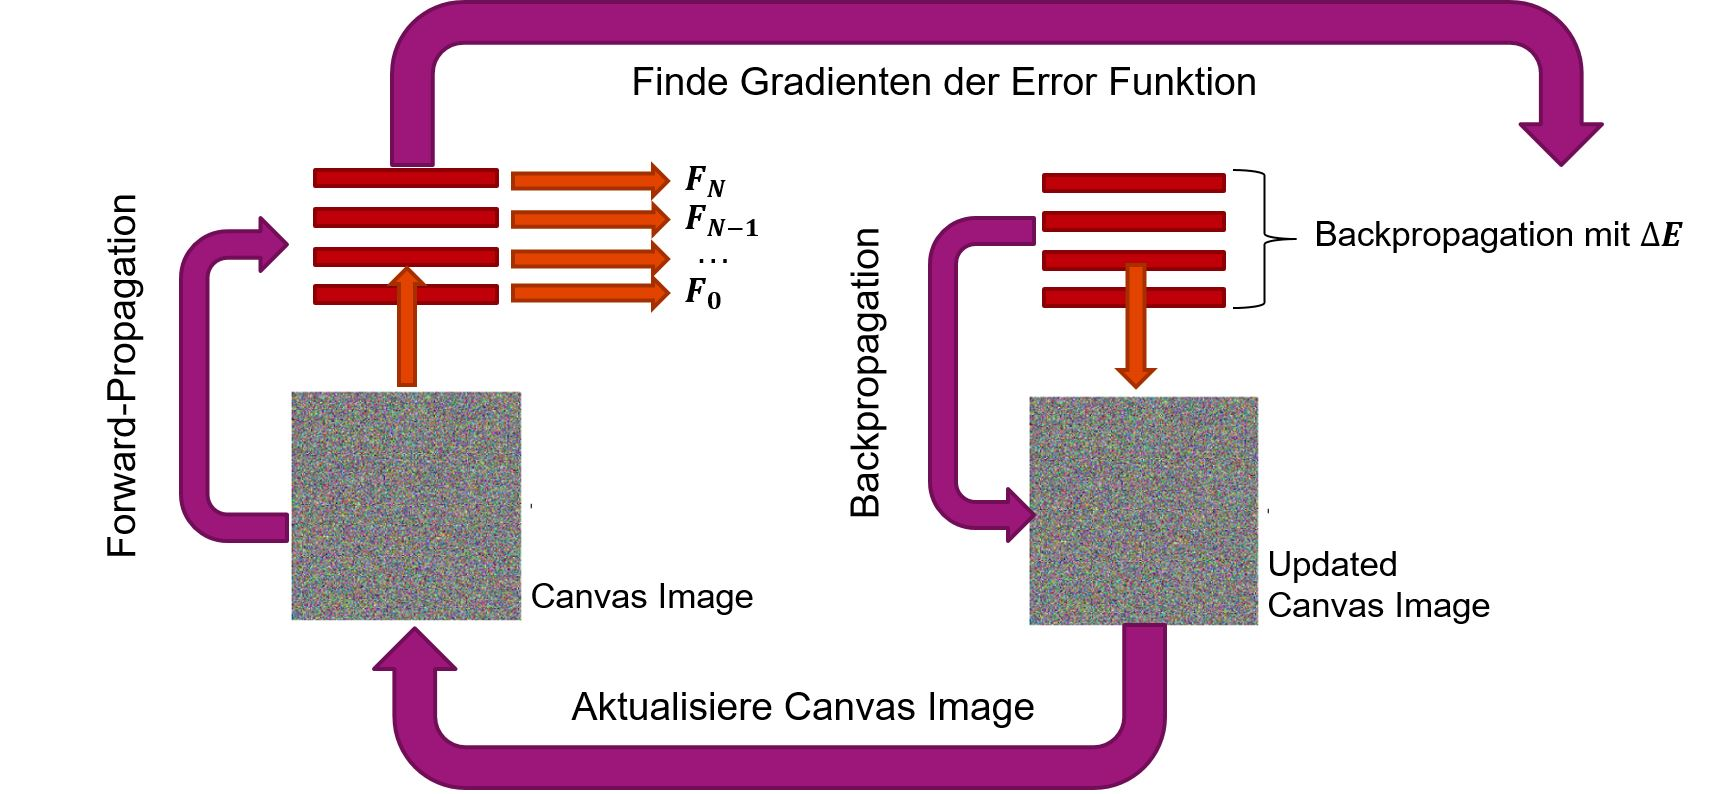
\includegraphics[width=\columnwidth]{Bilder/DeepStyle.jpg}
	\caption{Ablaufdiagramm des Deep Style Verfahrens.}
	\label{fig:DeepStyle}
\end{figure}
\footnotesize
\begin{equation}
F_{con}(\vec{f_{GC}}, \vec{f})= \frac{1}{2}\sum_{i,j}\vec{GC_{ij}}- \vec{f_{ij}})^2
\label{eq:DeepStyleContError}
\end{equation}
\small

\footnotesize
\begin{equation}
G_{ij}^N= \frac{1}{2}\sum_{k=0}^N (\vec{f_{ik}}- \vec{f_{jk}})^2
\label{eq:DeepStyleCorr}
\end{equation}
\small

\footnotesize
\begin{equation}
F_N= \frac{1}{2N_l^2M_l^2}\sum_{k=0}^N (G_{ij}^N- \vec{GS_{ij}^N})^2
\label{eq:DeepStyleCorrErr}
\end{equation}
\small

\footnotesize
\begin{equation}
F_{style}(SS,CI)= \sum_{k=0}^N w_l F_k
\label{eq:DeepStyleCorrErr}
\end{equation}
\small

\footnotesize
\begin{equation}
F_(SS,CS,CI)= \alpha F_{con}+\beta F_{style}
\label{eq:DeepStyleCorrErr}
\end{equation}
\small

\begin{figure}
	\flushleft
	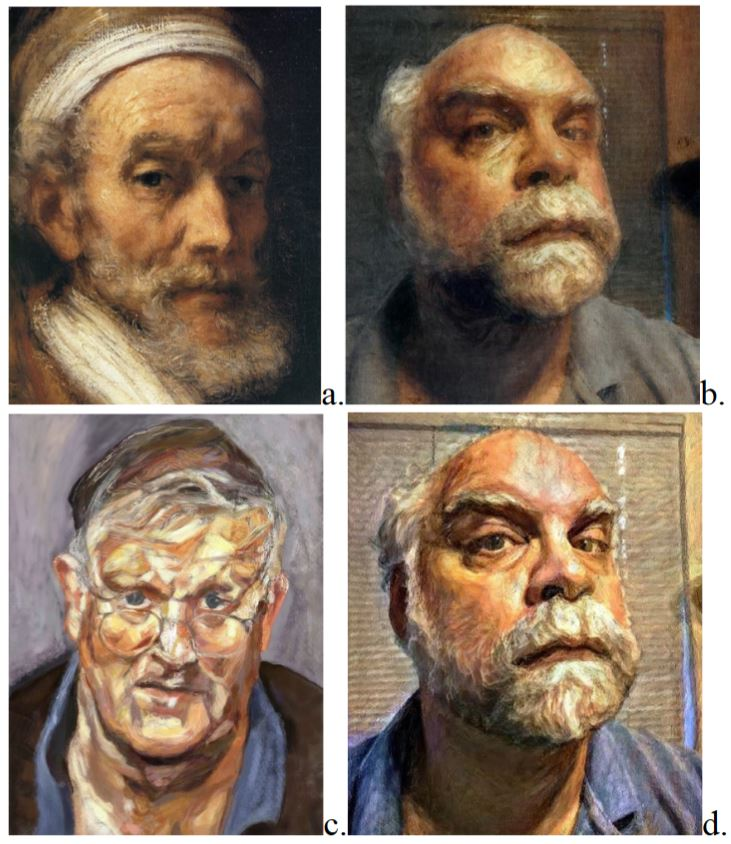
\includegraphics[width=\columnwidth]{Bilder/DeepStyleResults.JPG}
	\caption{Resultate des Deep Style Verfahrens~\cite{McCaigDG16}.}
	\label{fig:DeepStyleResults}
\end{figure}

\SubSection{Ausblick}

In der Zukunft kann das \textit{Deep Style} Verfahren für verschiedene Anwendungen sinnvoll sein. Zunächst sei hier die qualitativ hochwertige und automatische Coloration und Texturierung von animierten Filmen ohne die aufwendige manuelle Texturierung von einzelnen 3D Objekten. \\
Die Rekonstruktion und Restauration von verlorenen Filmmaterial, wie zum Beispiel \textit{Metropolis} von Fritz Lang ist vorstellbar. Da verlorene Szenen nachgestellt werden könnten und an den Stil der verbliebenen Szenen angepasst werden.\\
Auch eine individuelle Anpassung an den Geschmack und Stimmung des Nutzers von Filmen ist für \textit{Video-on-Demand} denkbar. Gerade die Farbgebung beeinflusst die Wahrnehmung des Zuschauers. So könnte zum Beispiel die Bedrohlichkeit eines Thrillers verschärft oder minimiert werden. Dasselbe gilt auch für Computerspiele, welche unter Umständen an Geschmack von jüngerem oder erwachsenem Publikum angepasst werden könnte.

\Section{Fazit} \label{Fazit}
\todo[inline, color=red]{Vera} 



\newpage
\Urlmuskip=0mu plus 1mu\relax %Bricht Link in Bibfile um
\bibliographystyle{latex8} 
\bibliography{psm}

\end{document}

